\usetikzlibrary{trees,shadows}
\providecommand{\imagewidth}{\textwidth}
\begin{tikzpicture}[
 line width=1.2,
variablenode/.style={circle,draw=red,fill=white,thick}]

% draw image
\node[anchor=south west,inner sep=0] (image) at (0,0)
{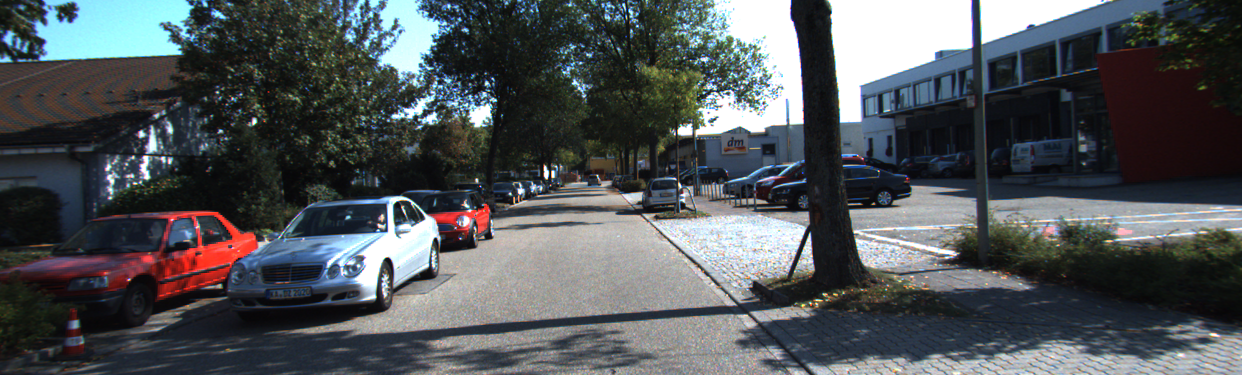
\includegraphics[width=\imagewidth]{graphics/0000000061_raw.png}};

    \begin{scope}[x={(image.south east)},y={(image.north west)}]
		\path (0.05, 0.3) node [variablenode] (x6) {\large{6}}
				    (0.25, 0.3) node [variablenode] (x2) {\large{2}}
				    (0.41, 0.45) node [variablenode,inner sep=3] (x1) {\tiny{1}}
				    (0.36, 0.39) node [variablenode,inner sep=3] (x5) {\small{5}}
				    (0.55, 0.4) node [variablenode,inner sep=3] (x3) {\small{3}}
					(0.63, 0.49) node [variablenode,inner sep=3] (x4) {\tiny{4}}
;
\draw (x6) -- (x2);
\draw (x5) -- (x2);
\draw (x1) -- (x5);
    \end{scope}
\end{tikzpicture}
